\PassOptionsToPackage{unicode=true}{hyperref} % options for packages loaded elsewhere
\PassOptionsToPackage{hyphens}{url}
%
\documentclass[
]{article}
\usepackage{lmodern}
\usepackage{amssymb,amsmath}
\usepackage{ifxetex,ifluatex}
\ifnum 0\ifxetex 1\fi\ifluatex 1\fi=0 % if pdftex
  \usepackage[T1]{fontenc}
  \usepackage[utf8]{inputenc}
  \usepackage{textcomp} % provides euro and other symbols
\else % if luatex or xelatex
  \usepackage{unicode-math}
  \defaultfontfeatures{Scale=MatchLowercase}
  \defaultfontfeatures[\rmfamily]{Ligatures=TeX,Scale=1}
\fi
% use upquote if available, for straight quotes in verbatim environments
\IfFileExists{upquote.sty}{\usepackage{upquote}}{}
\IfFileExists{microtype.sty}{% use microtype if available
  \usepackage[]{microtype}
  \UseMicrotypeSet[protrusion]{basicmath} % disable protrusion for tt fonts
}{}
\makeatletter
\@ifundefined{KOMAClassName}{% if non-KOMA class
  \IfFileExists{parskip.sty}{%
    \usepackage{parskip}
  }{% else
    \setlength{\parindent}{0pt}
    \setlength{\parskip}{6pt plus 2pt minus 1pt}}
}{% if KOMA class
  \KOMAoptions{parskip=half}}
\makeatother
\usepackage{xcolor}
\IfFileExists{xurl.sty}{\usepackage{xurl}}{} % add URL line breaks if available
\IfFileExists{bookmark.sty}{\usepackage{bookmark}}{\usepackage{hyperref}}
\hypersetup{
  pdfborder={0 0 0},
  breaklinks=true}
\urlstyle{same}  % don't use monospace font for urls
\usepackage{graphicx,grffile}
\usepackage[english]{babel}

\makeatletter
\def\maxwidth{\ifdim\Gin@nat@width>\linewidth\linewidth\else\Gin@nat@width\fi}
\def\maxheight{\ifdim\Gin@nat@height>\textheight\textheight\else\Gin@nat@height\fi}
\makeatother
% Scale images if necessary, so that they will not overflow the page
% margins by default, and it is still possible to overwrite the defaults
% using explicit options in \includegraphics[width, height, ...]{}
\setkeys{Gin}{width=\maxwidth,height=\maxheight,keepaspectratio}
\setlength{\emergencystretch}{3em}  % prevent overfull lines
\providecommand{\tightlist}{%
  \setlength{\itemsep}{0pt}\setlength{\parskip}{0pt}}
\setcounter{secnumdepth}{-2}
% Redefines (sub)paragraphs to behave more like sections
\ifx\paragraph\undefined\else
  \let\oldparagraph\paragraph
  \renewcommand{\paragraph}[1]{\oldparagraph{#1}\mbox{}}
\fi
\ifx\subparagraph\undefined\else
  \let\oldsubparagraph\subparagraph
  \renewcommand{\subparagraph}[1]{\oldsubparagraph{#1}\mbox{}}
\fi

% set default figure placement to htbp
\makeatletter
\def\fps@figure{htbp}
\makeatother


\date{}

\begin{document}

I have worked on two tasks:

\begin{enumerate}
\def\labelenumi{\arabic{enumi}.}
\tightlist
\item
  Generating maximal candidates
\item
  Optimizing the selection of candidates
\end{enumerate}

\textbf{Generating maximal candidates.} Given a board with defects, the
goal of this task is to enumerate all the maximal empty rectangles. A
\emph{maximal empty rectangle} (MER) is defined as a rectangle
containing no defects and not included in any other defect-free
rectangle. Both the board and the defects are represented as rectangles
and the data is randomly generated (but we could also use the
annotations from various datasets; \emph{e.g.}, Salum, Oulu).

Here is an example of a board (in blue) and defects (in red): \\
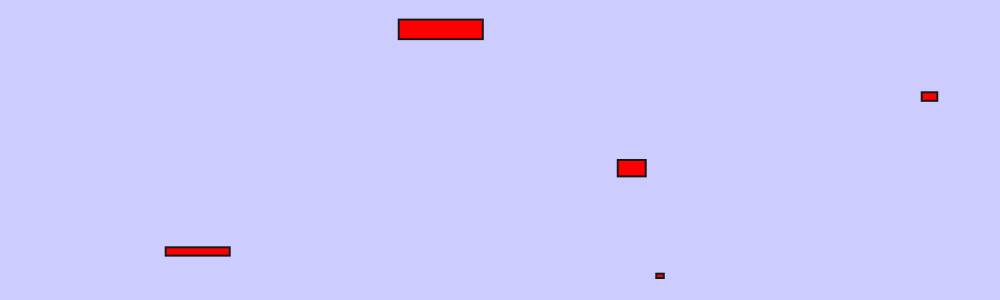
\includegraphics{imgs/board.png}

And here are candidate MERs of different types:

\begin{itemize}
\tightlist
\item
  delimited by two opposite sides of the boards (top-bottom and
  left-right) \\
  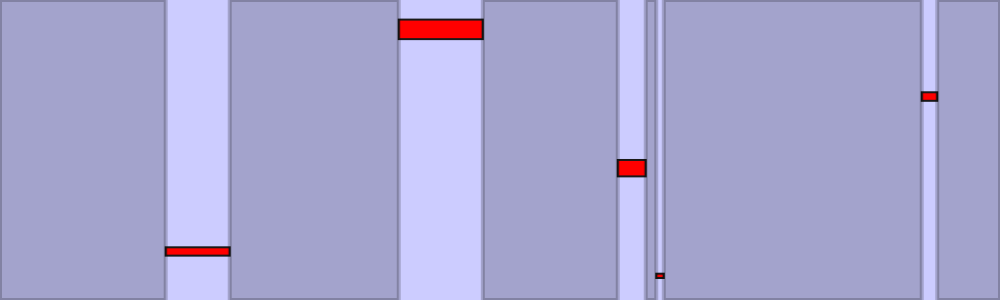
\includegraphics{imgs/mers-1a.png}
  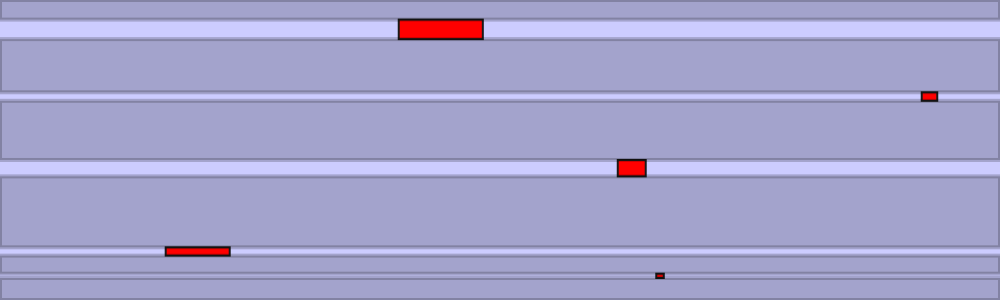
\includegraphics{imgs/mers-1b.png}
\item
  delimited by two adjacent sides of the boards \\
  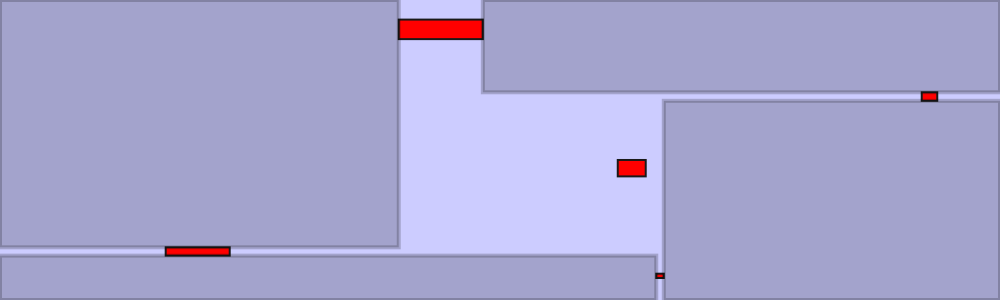
\includegraphics{imgs/mers-2.png}
\item
  delimited by one side of the board (top, left, bottom, right) \\
  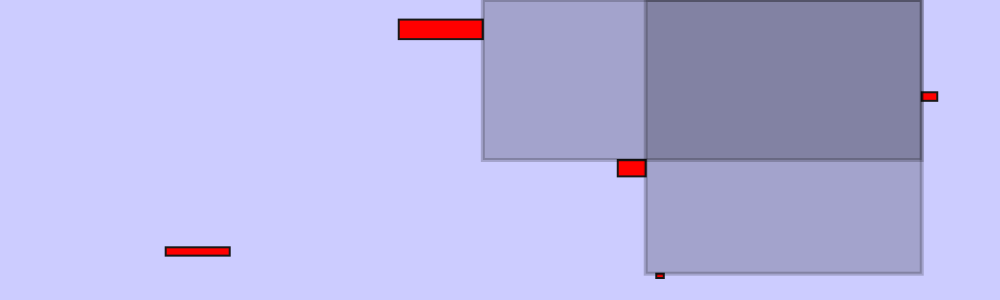
\includegraphics{imgs/mers-3a.png} 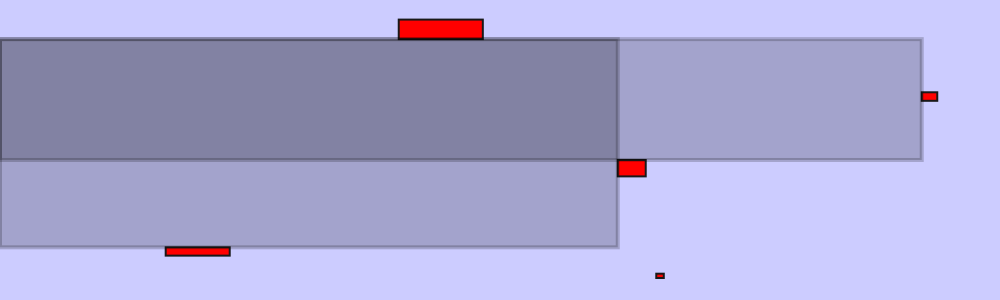
\includegraphics{imgs/mers-3b.png}
  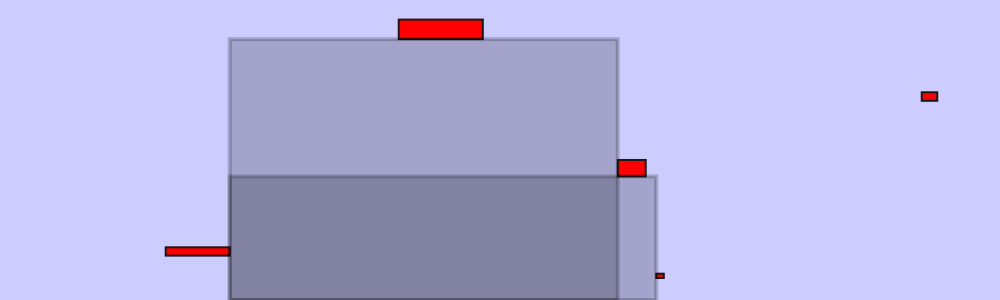
\includegraphics{imgs/mers-3c.png} 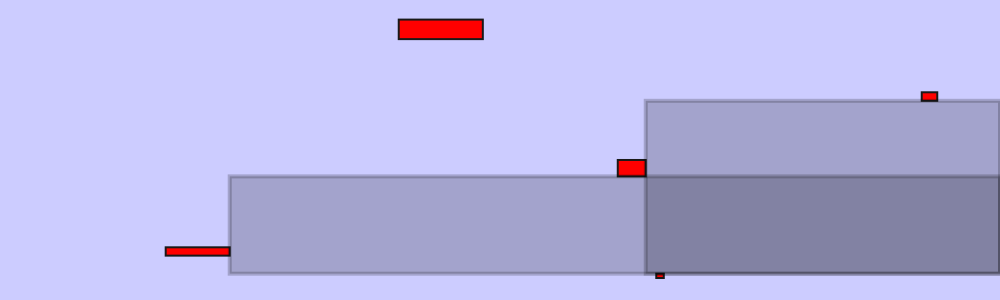
\includegraphics{imgs/mers-3d.png}
\end{itemize}

The code for this part is available
\href{https://bitbucket.org/doneata/optim-cut/src/master/candidates.py}{here}.

\textbf{Optimizing the selection of candidates.} The goal is to select
the candidate rectangles such \emph{(i)} the area they cover is
maximized and \emph{(ii)} any two rectangles do not overlap. To do this
we want to optimize the following problem:

\[
\begin{aligned}
\underset{\mathbf{x}}{\text{maximize}} \;\; & \mathbf{w}^\intercal\mathbf{x} \\
\text{subject to} \;\; &  x_i \in \left\{0, 1\right\}, \forall i \\
                       & \mathbf{x}^\intercal \mathbf{A} \mathbf{x} = 0
\end{aligned}
\]

where

\begin{itemize}
\tightlist
\item
  \(\mathbf{x}\) indicates the selection of rectangles, that is,
  \(x_i = 1\) if we select the \(i\)-th rectangle and \(x_i = 0\)
  otherwise.
\item
  \(\mathbf{w}\) contains the area of each of the candidate rectangles.
\item
  \(\mathbf{A}\) is a binary matrix with \(A_{ij} = 1\) if rectangles
  \(i\) and \(j\) overlap and \(A_{ij} = 0\) otherwise.
\end{itemize}

To simplify the optimization problem, I modify it in two ways:
\emph{(i)} relax the problem to continuous domain; \emph{(ii)} move the
quadratic constraint into the objective function. The new optimization
problem is:

\[
\begin{aligned}
\underset{\mathbf{x}}{\text{maximize}} \;\; & \mathbf{w}^\intercal\mathbf{x} - \alpha \frac{1}{2} \mathbf{x}^\intercal \mathbf{A} \mathbf{x} \\
\text{subject to} \;\; &  x \ge 0, \forall i\\
                       & \|\mathbf{x}\|_1 = 1
\end{aligned}
\]

To solve this I'm using the \href{https://cvxopt.org}{\texttt{cvxopt}}
package from Python. However, currently I'm running into some numerical
issues that I need to look into. The code for this part is available
\href{https://bitbucket.org/doneata/optim-cut/src/master/cut_qp.py}{here}.

\end{document}
